\chapter{Annex}

This appendix gathers the measurement results of the main scenarios investigated
for the thesis. 

\begin{figure}[H]
     \subfigure{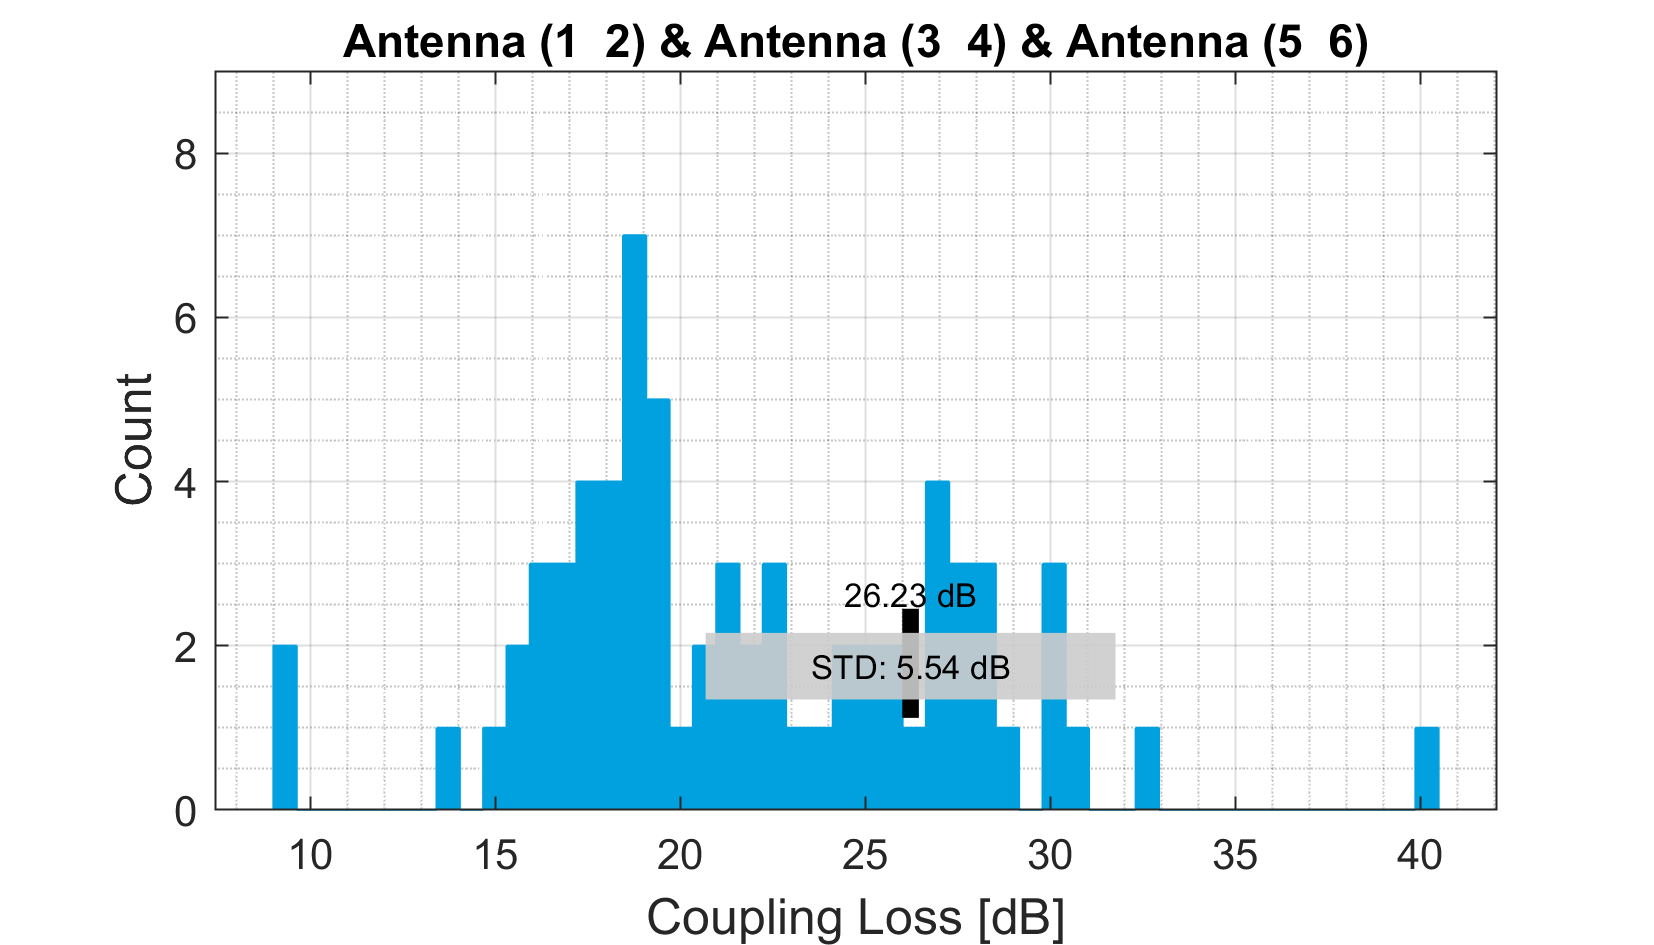
\includegraphics[scale = 0.37]{/Annex/Manual/plot1.png}} 
     \subfigure{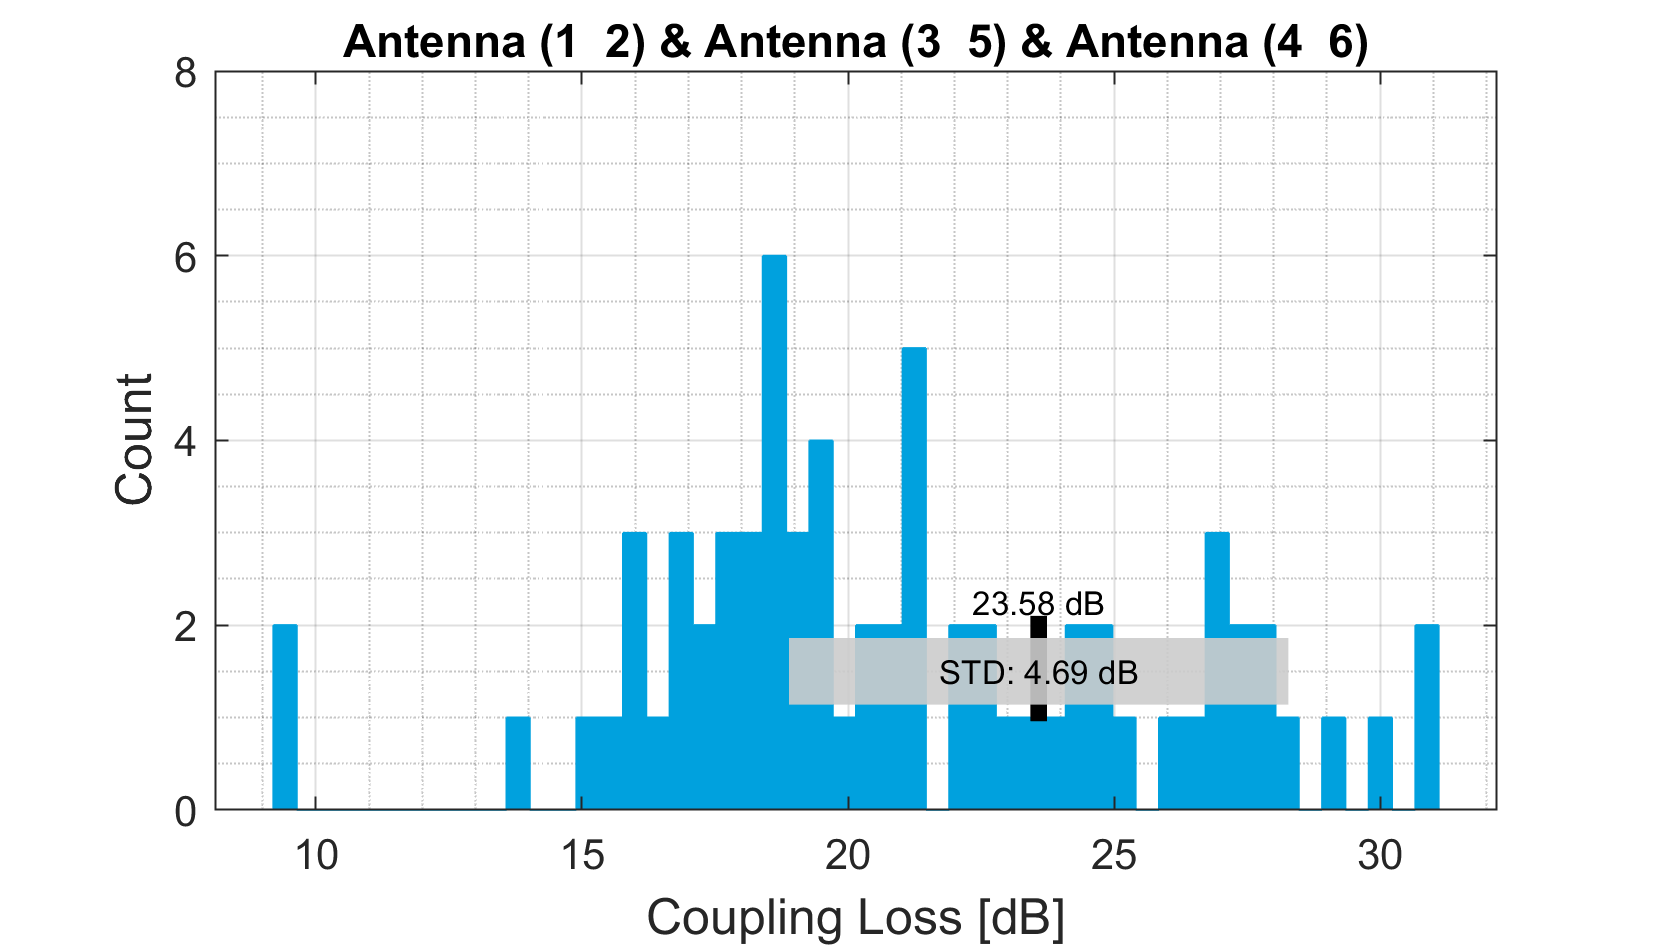
\includegraphics[scale = 0.37]{/Annex/Manual/plot2.png}} 
     \subfigure{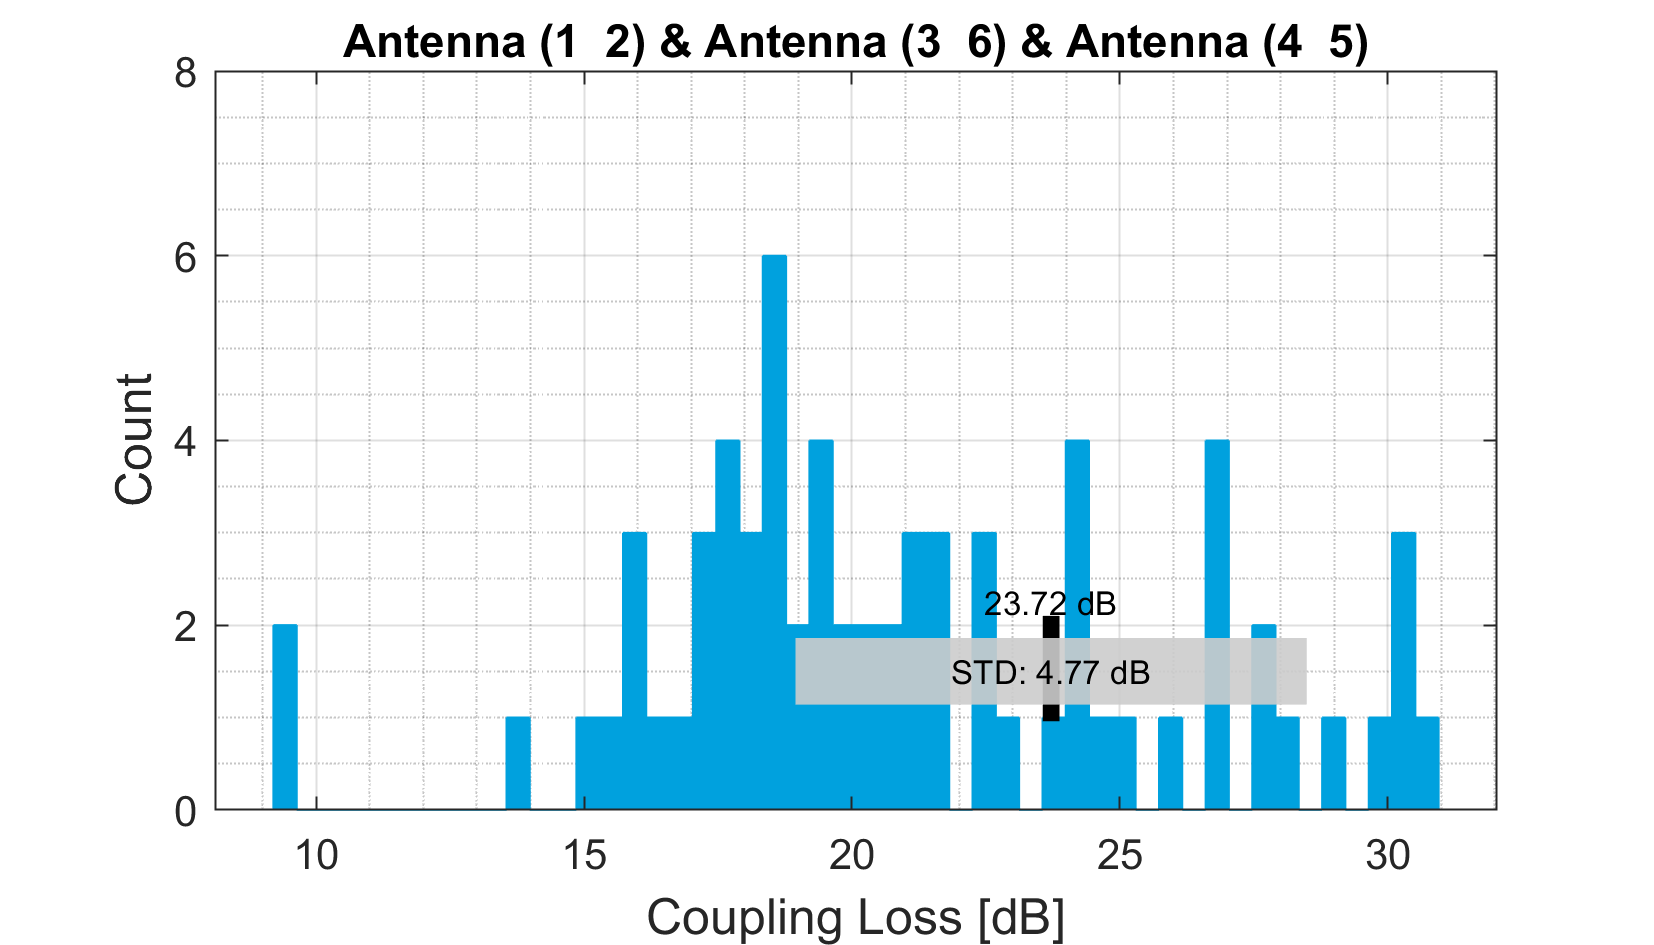
\includegraphics[scale = 0.37]{/Annex/Manual/plot3.png}}  \\
     \subfigure{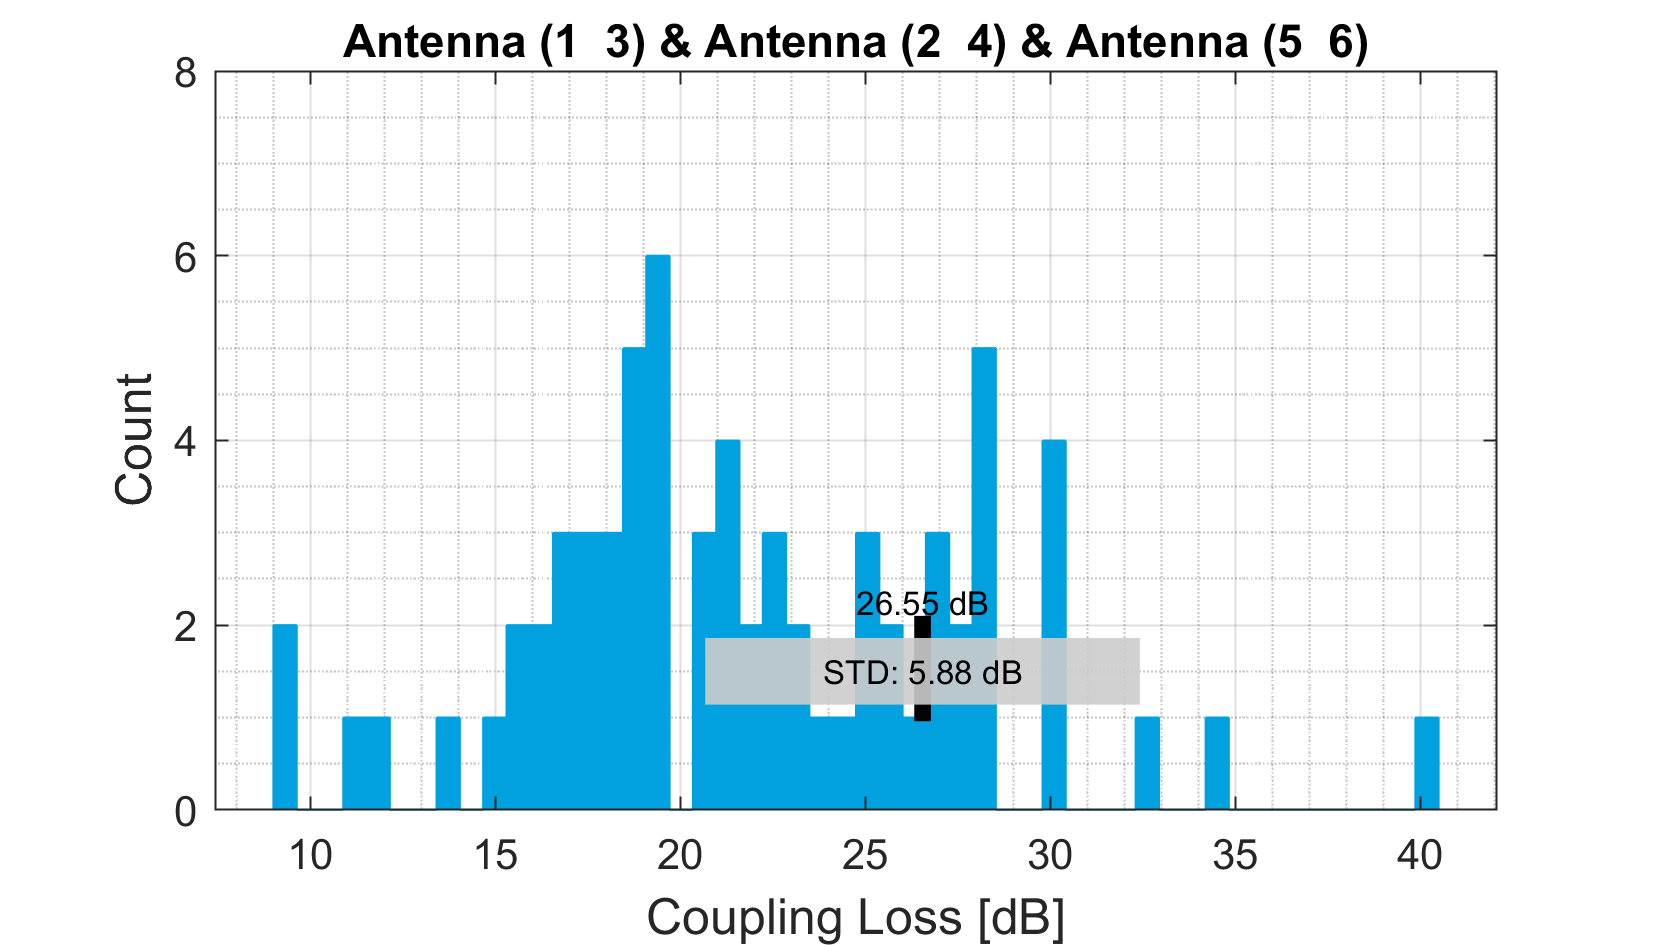
\includegraphics[scale = 0.37]{/Annex/Manual/plot4.png}} 
     \subfigure{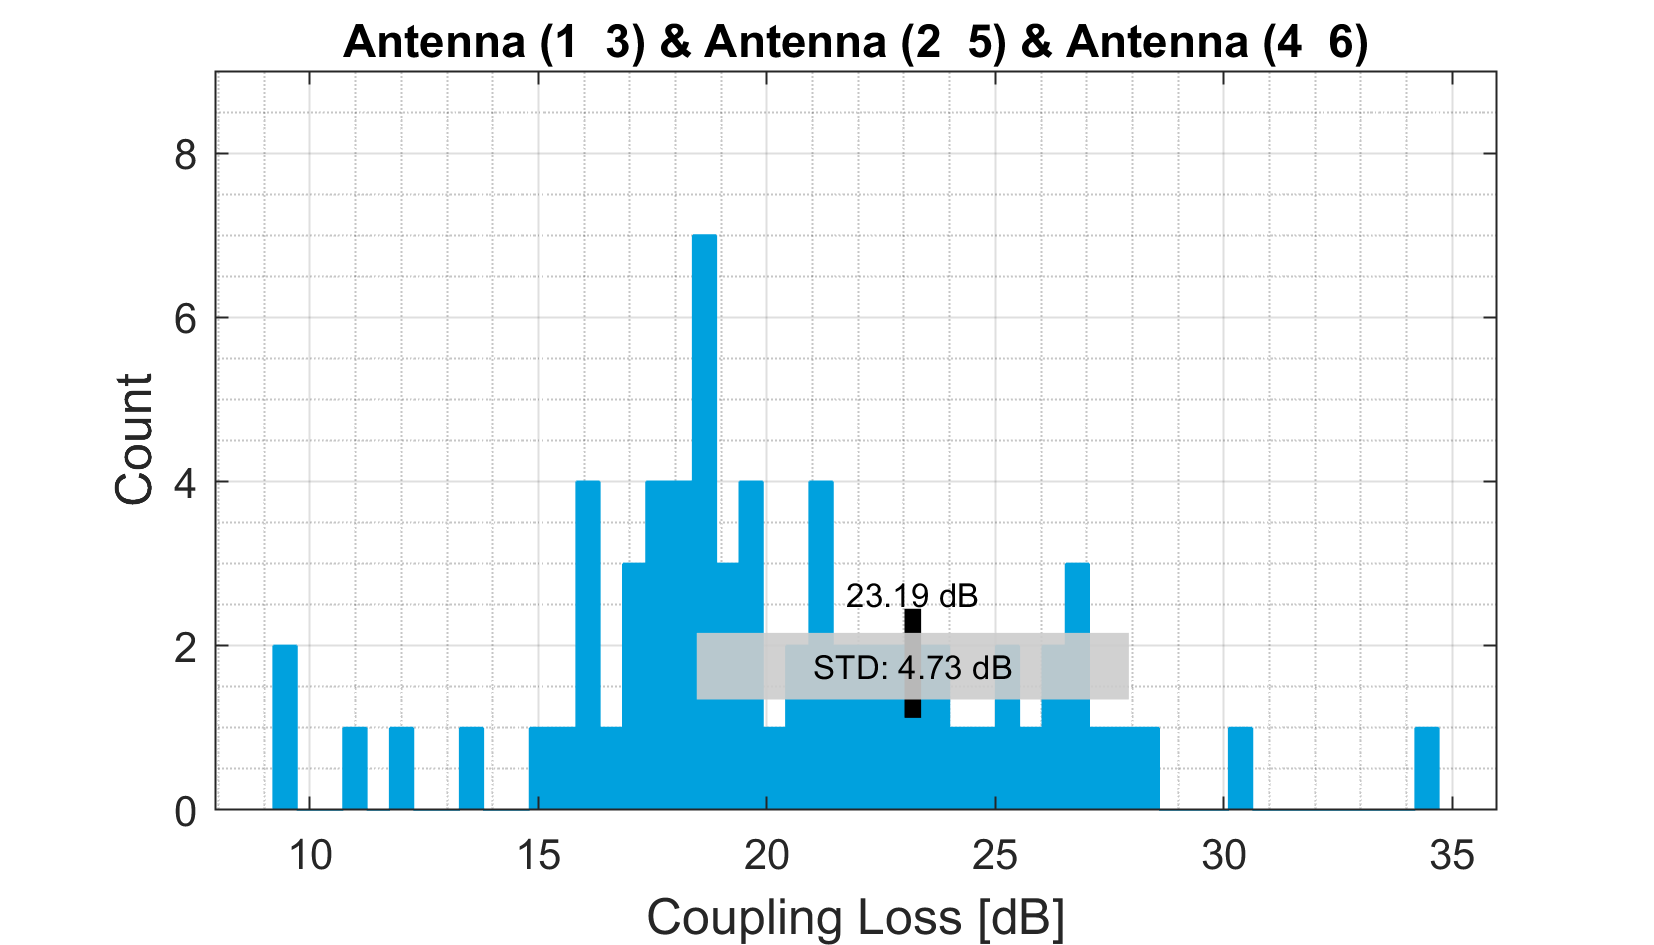
\includegraphics[scale = 0.37]{/Annex/Manual/plot5.png}} 
     \subfigure{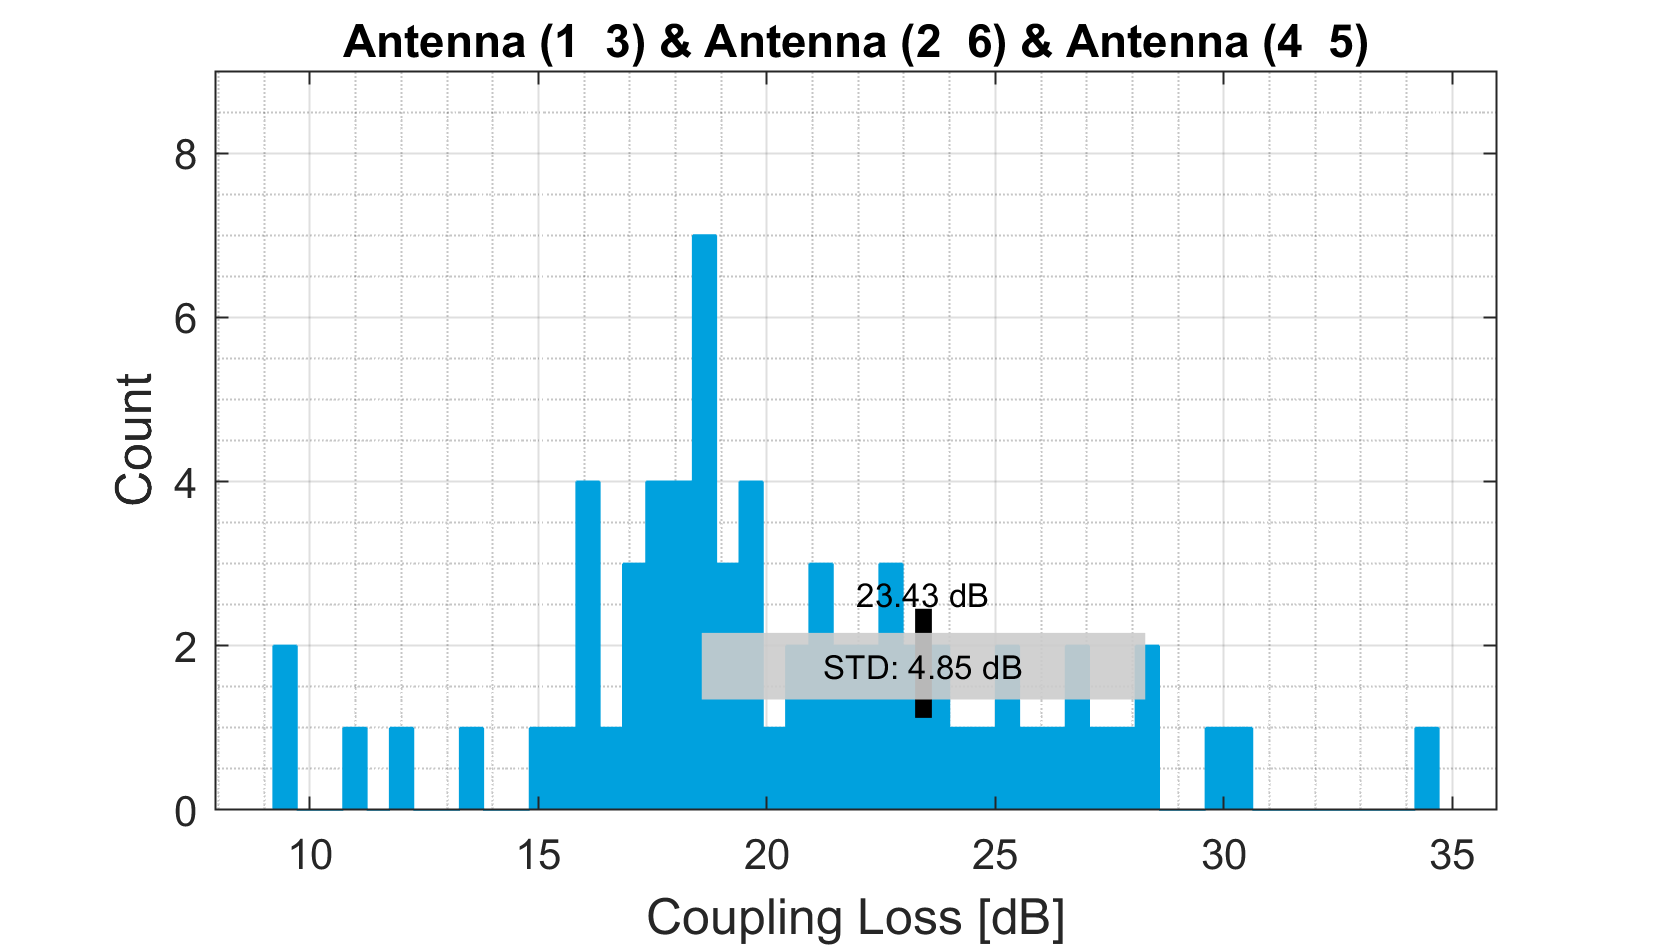
\includegraphics[scale = 0.37]{/Annex/Manual/plot6.png}}  \\
     \subfigure{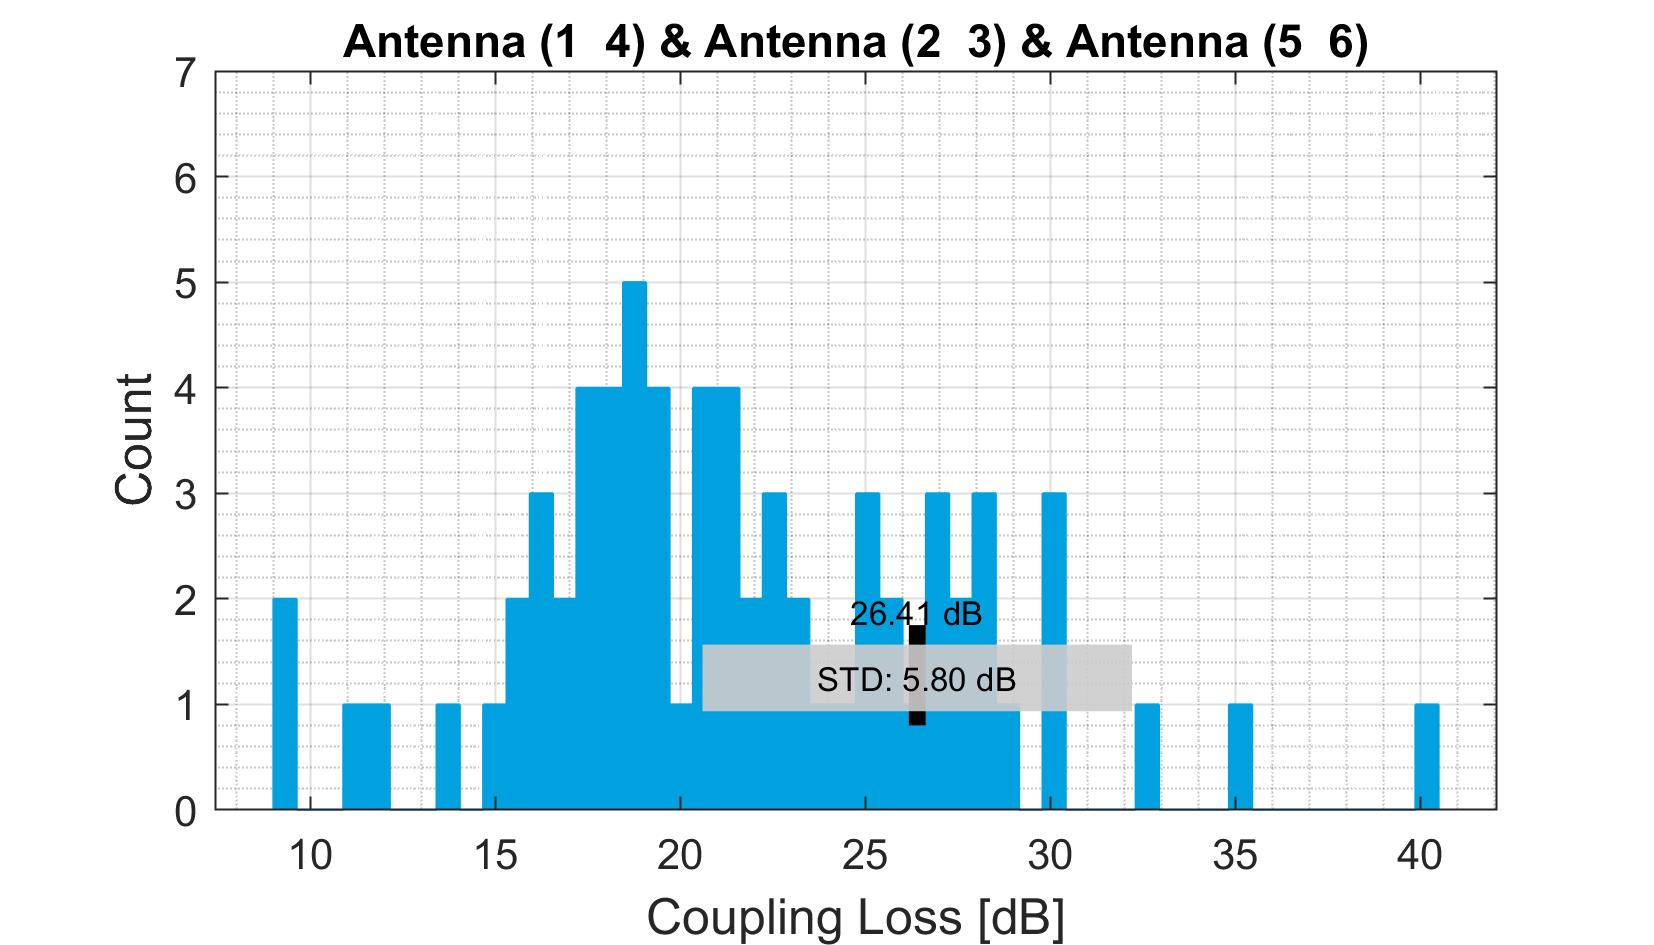
\includegraphics[scale = 0.37]{/Annex/Manual/plot7.png}} 
     \subfigure{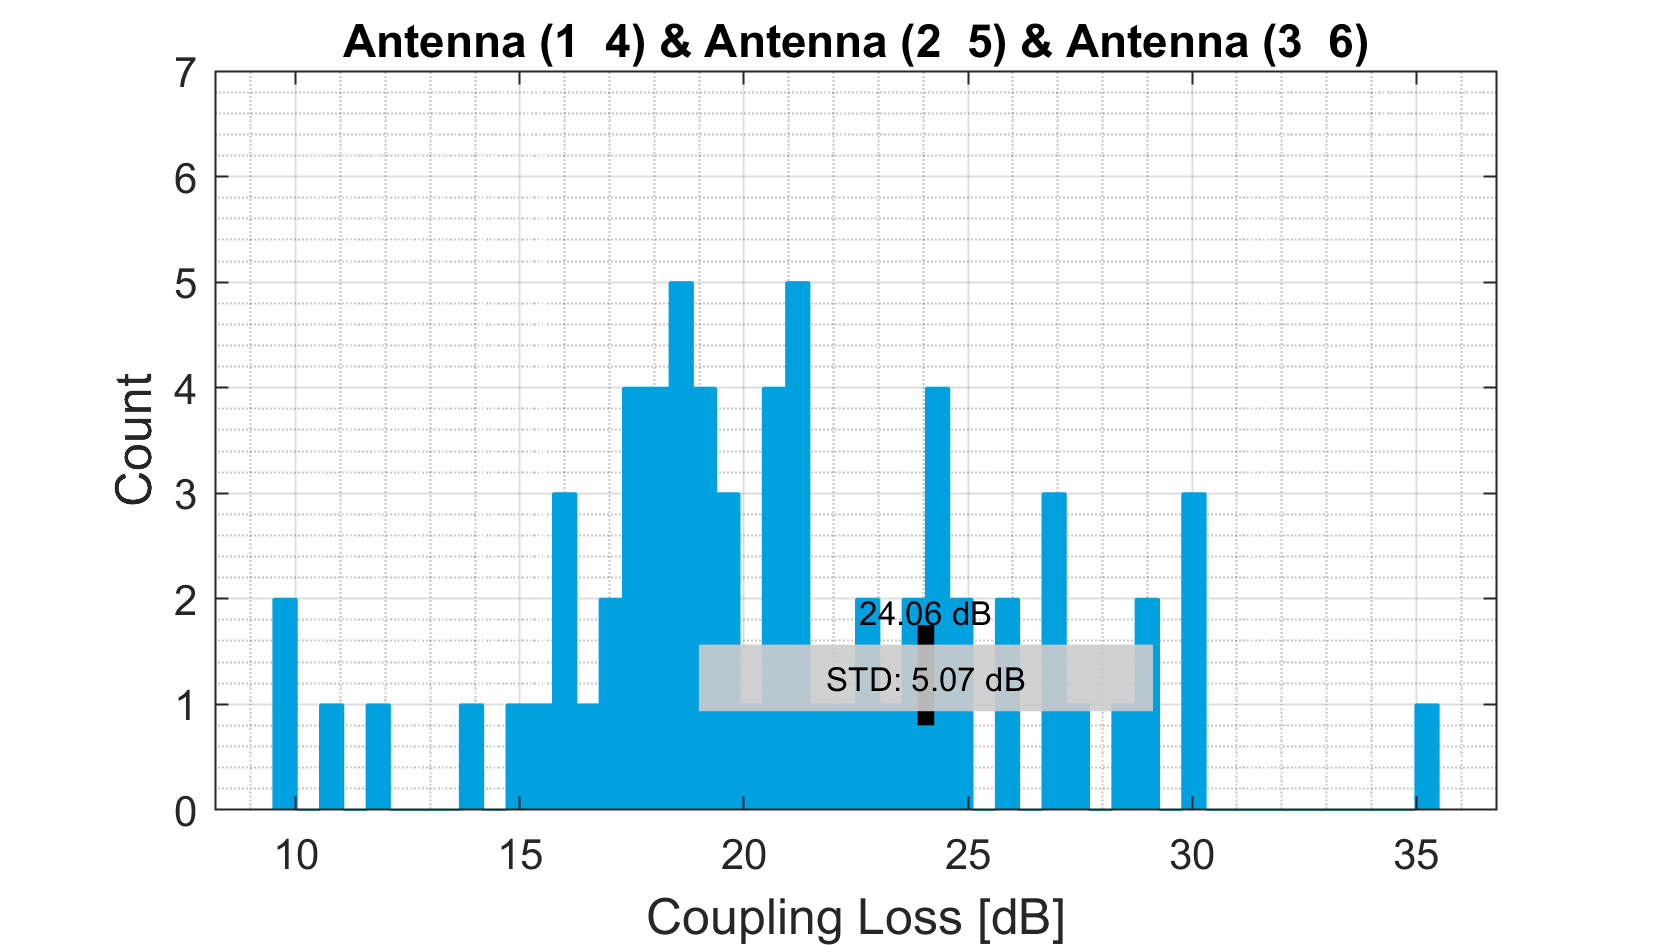
\includegraphics[scale = 0.37]{/Annex/Manual/plot8.png}} 
     \subfigure{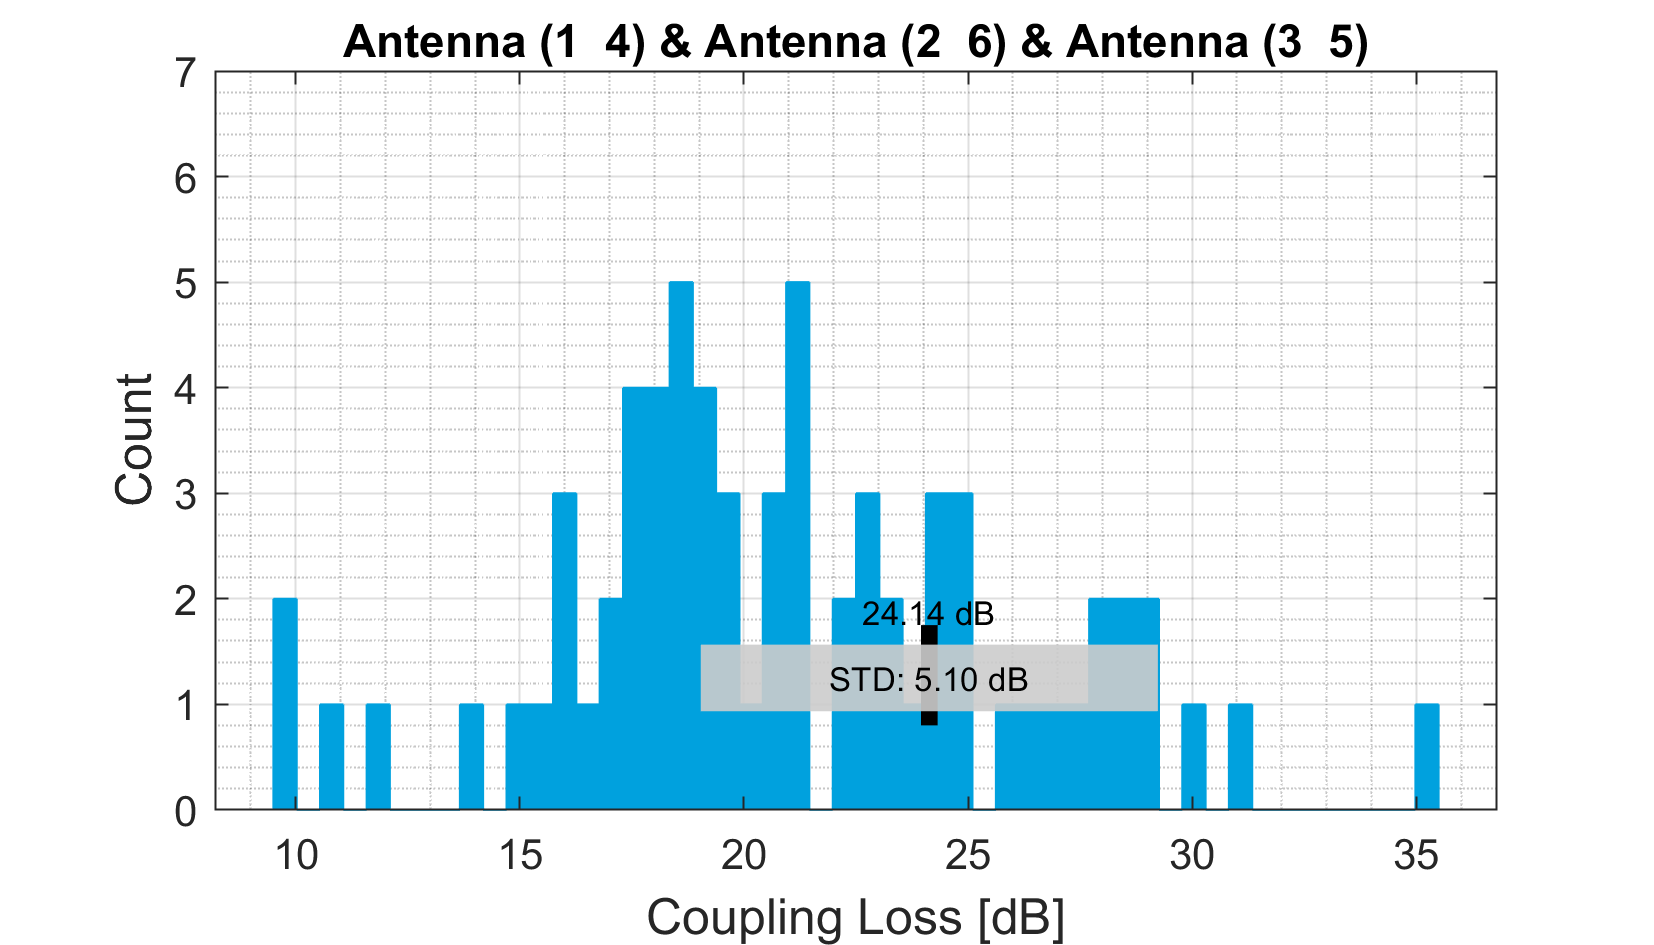
\includegraphics[scale = 0.37]{/Annex/Manual/plot9.png}}  \\
     \subfigure{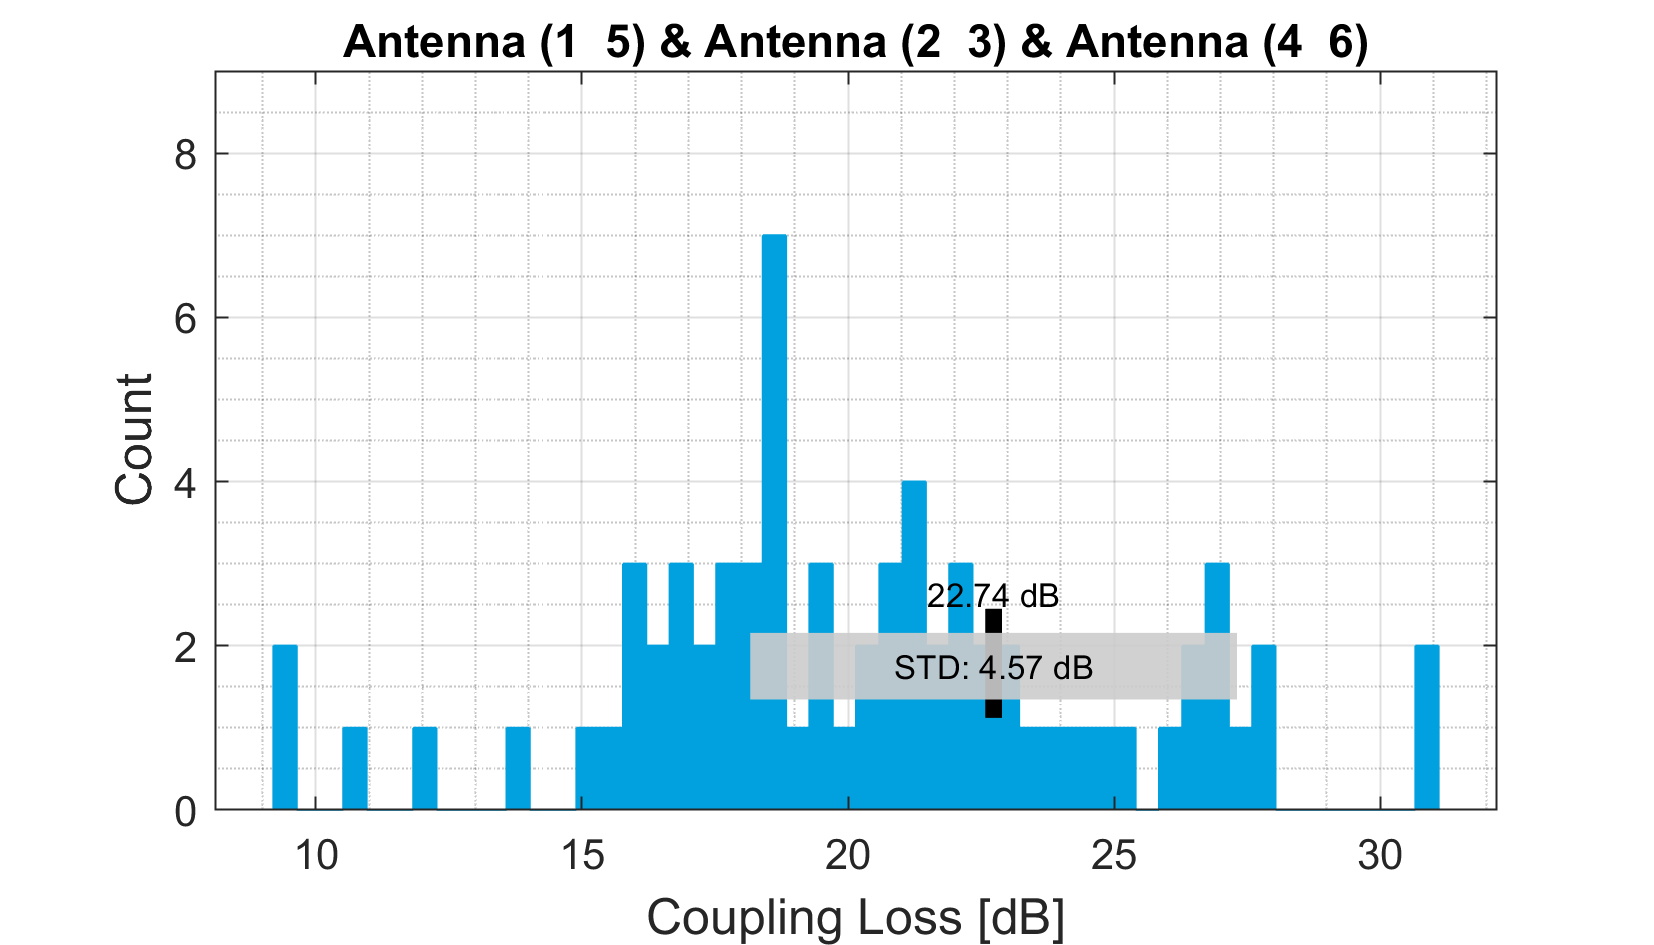
\includegraphics[scale = 0.37]{/Annex/Manual/plot10.png}} 
     \subfigure{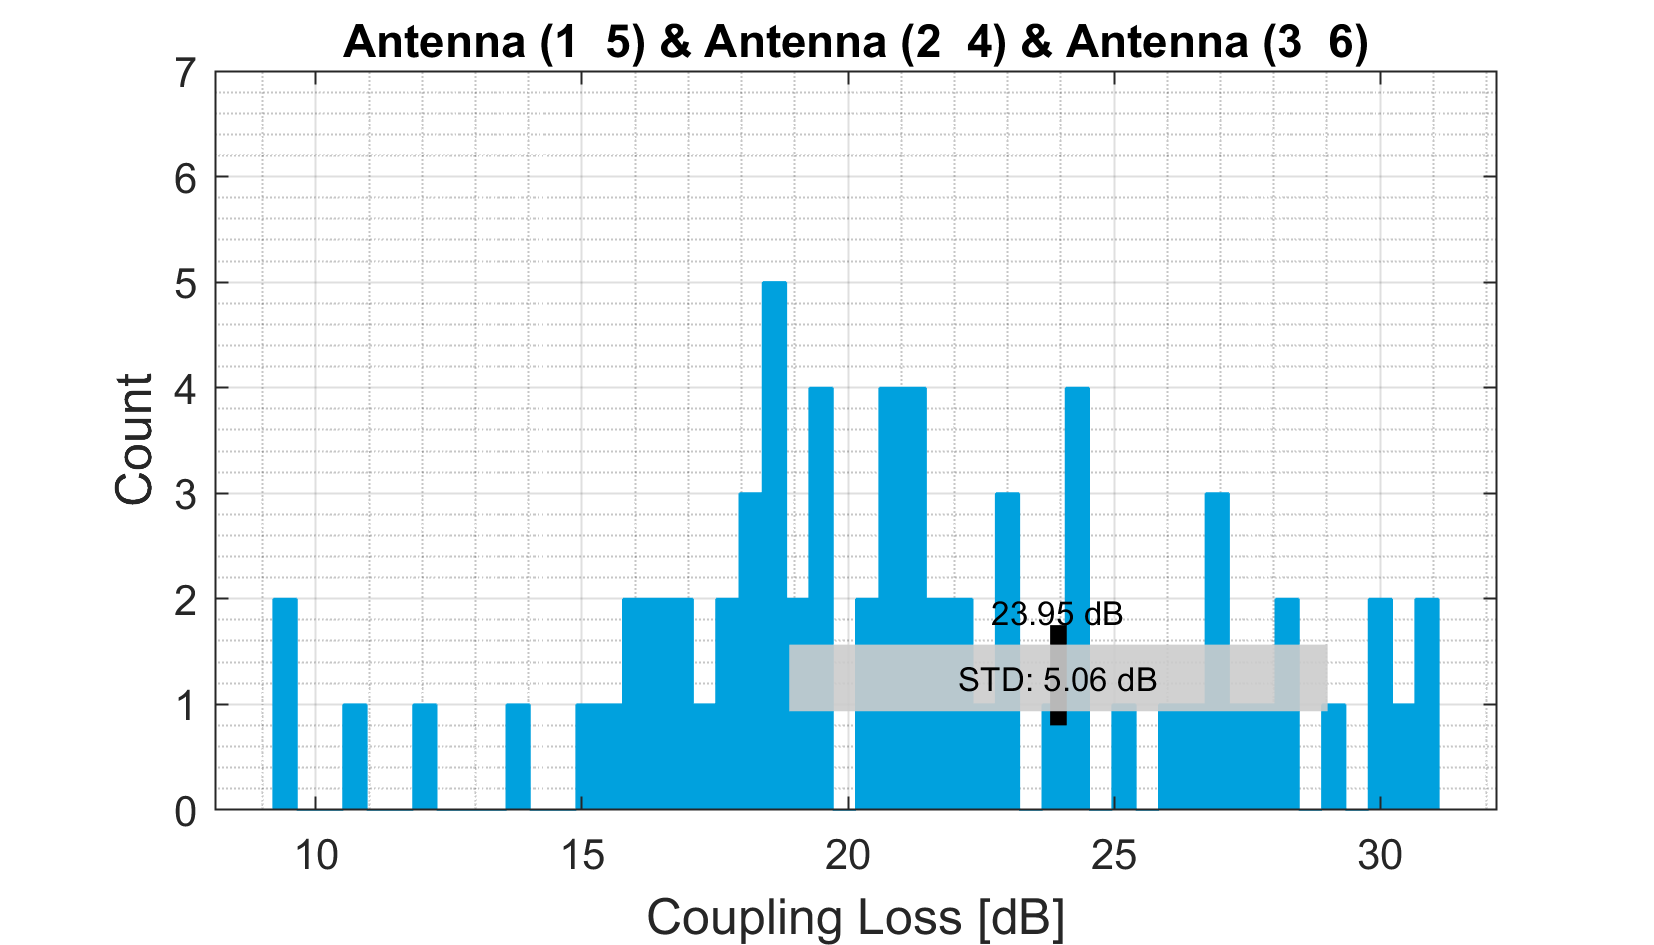
\includegraphics[scale = 0.37]{/Annex/Manual/plot11.png}} 
     \subfigure{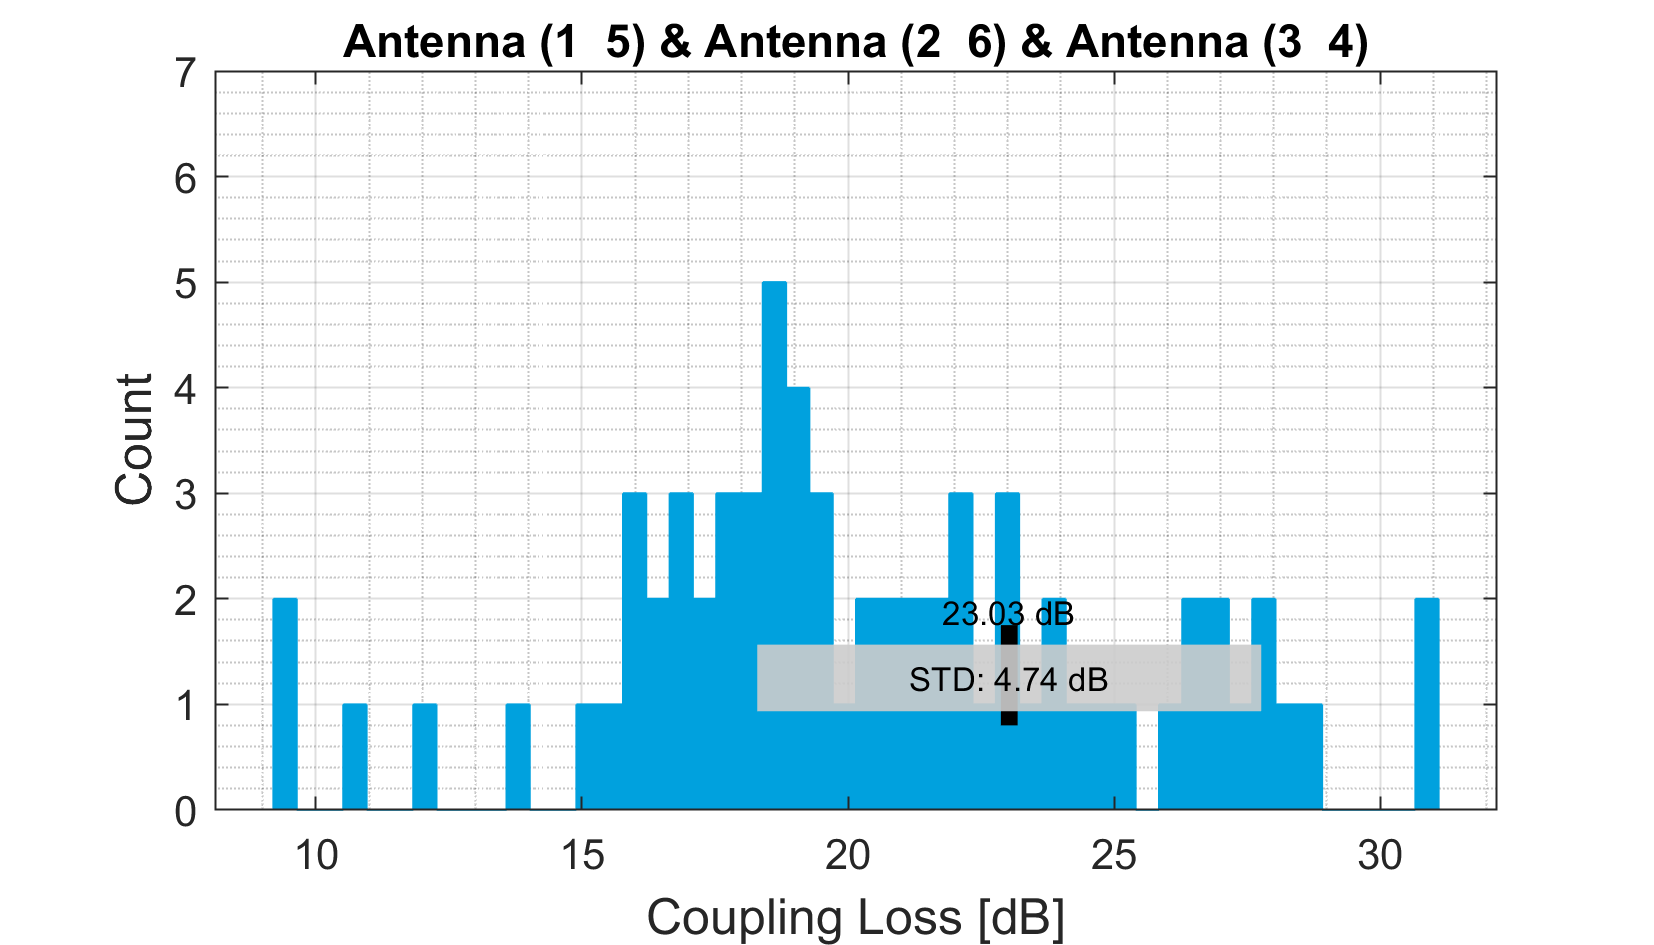
\includegraphics[scale = 0.37]{/Annex/Manual/plot12.png}}  \\
      \subfigure{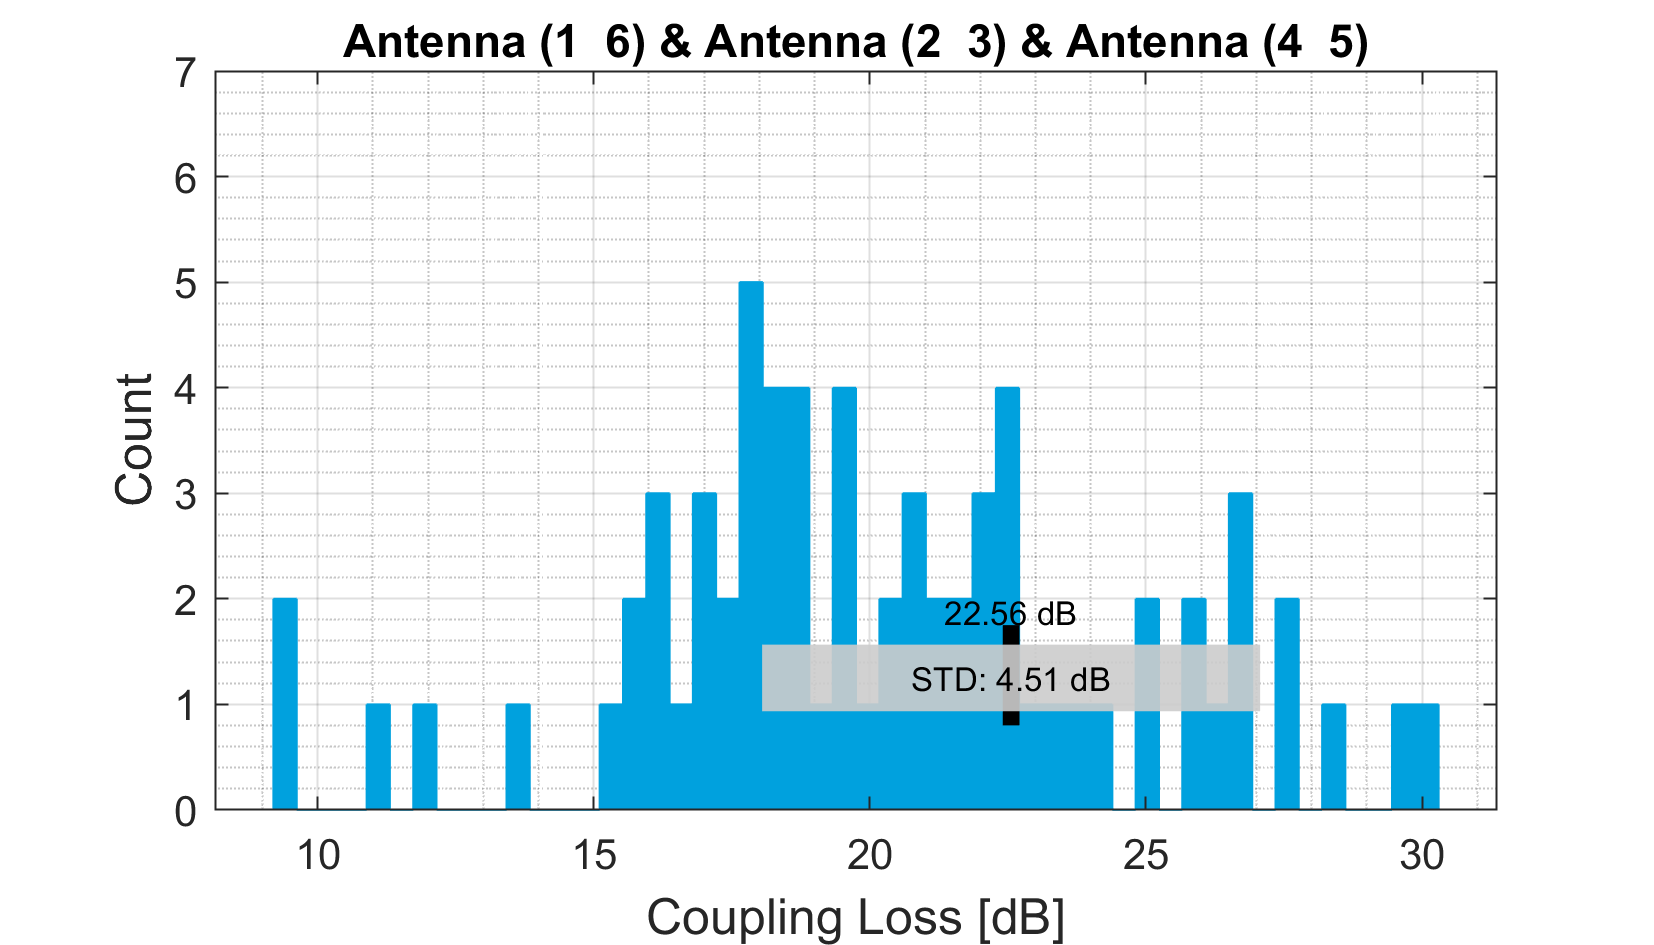
\includegraphics[scale = 0.37]{/Annex/Manual/plot13.png}} 
     \subfigure{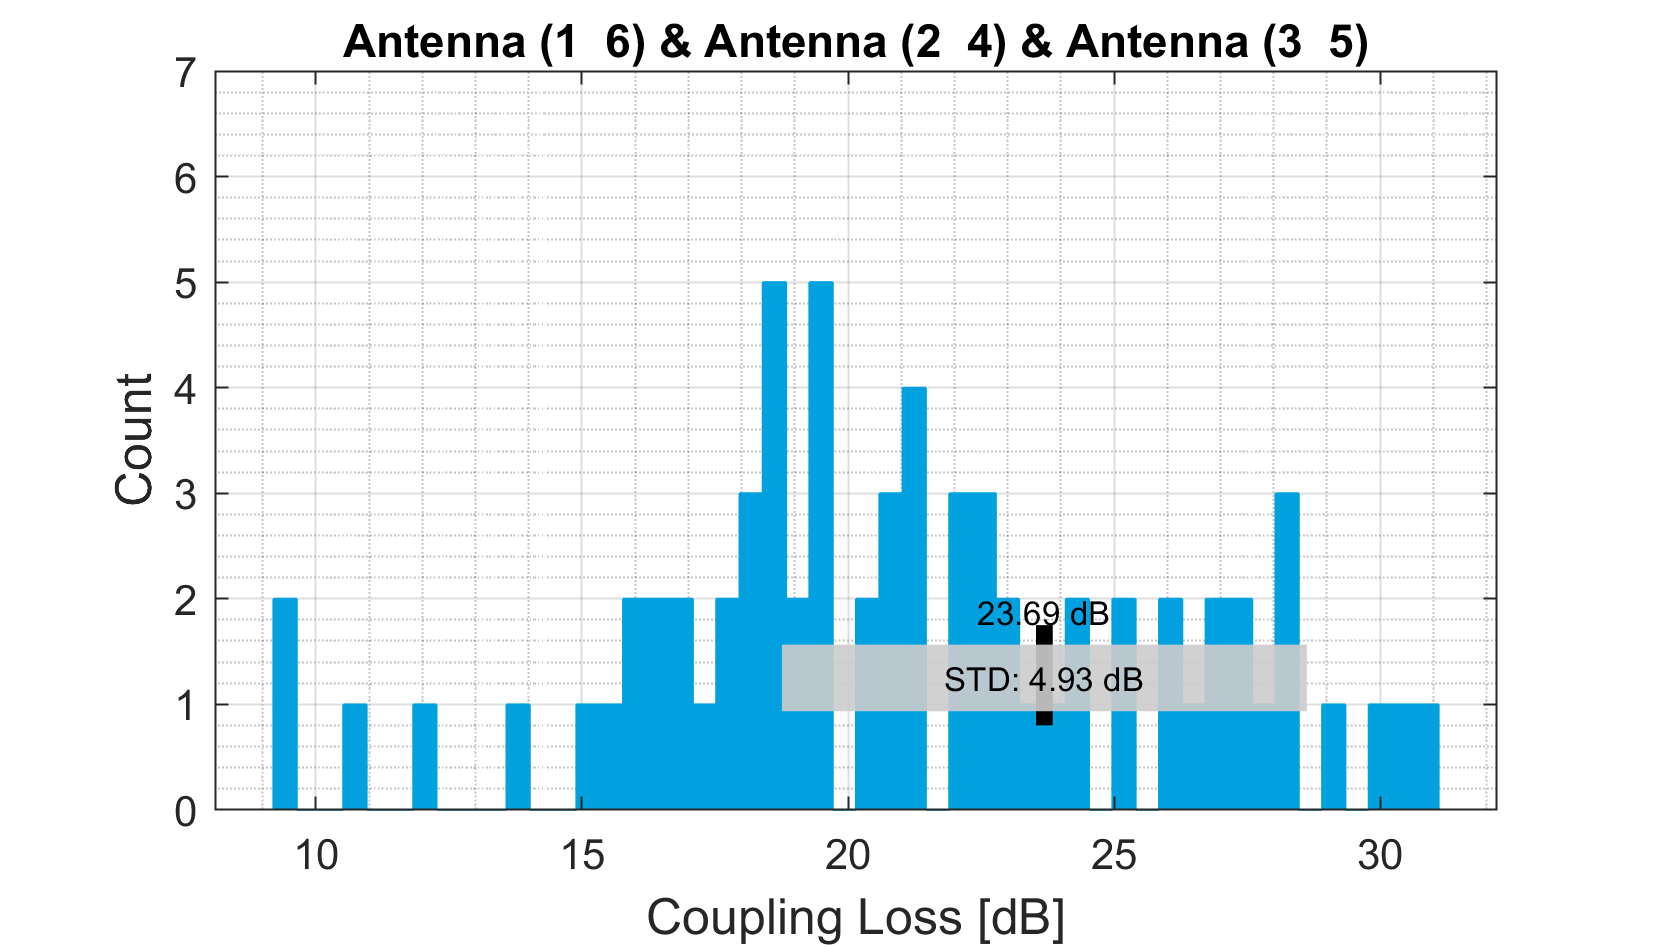
\includegraphics[scale = 0.37]{/Annex/Manual/plot14.png}} 
     \subfigure{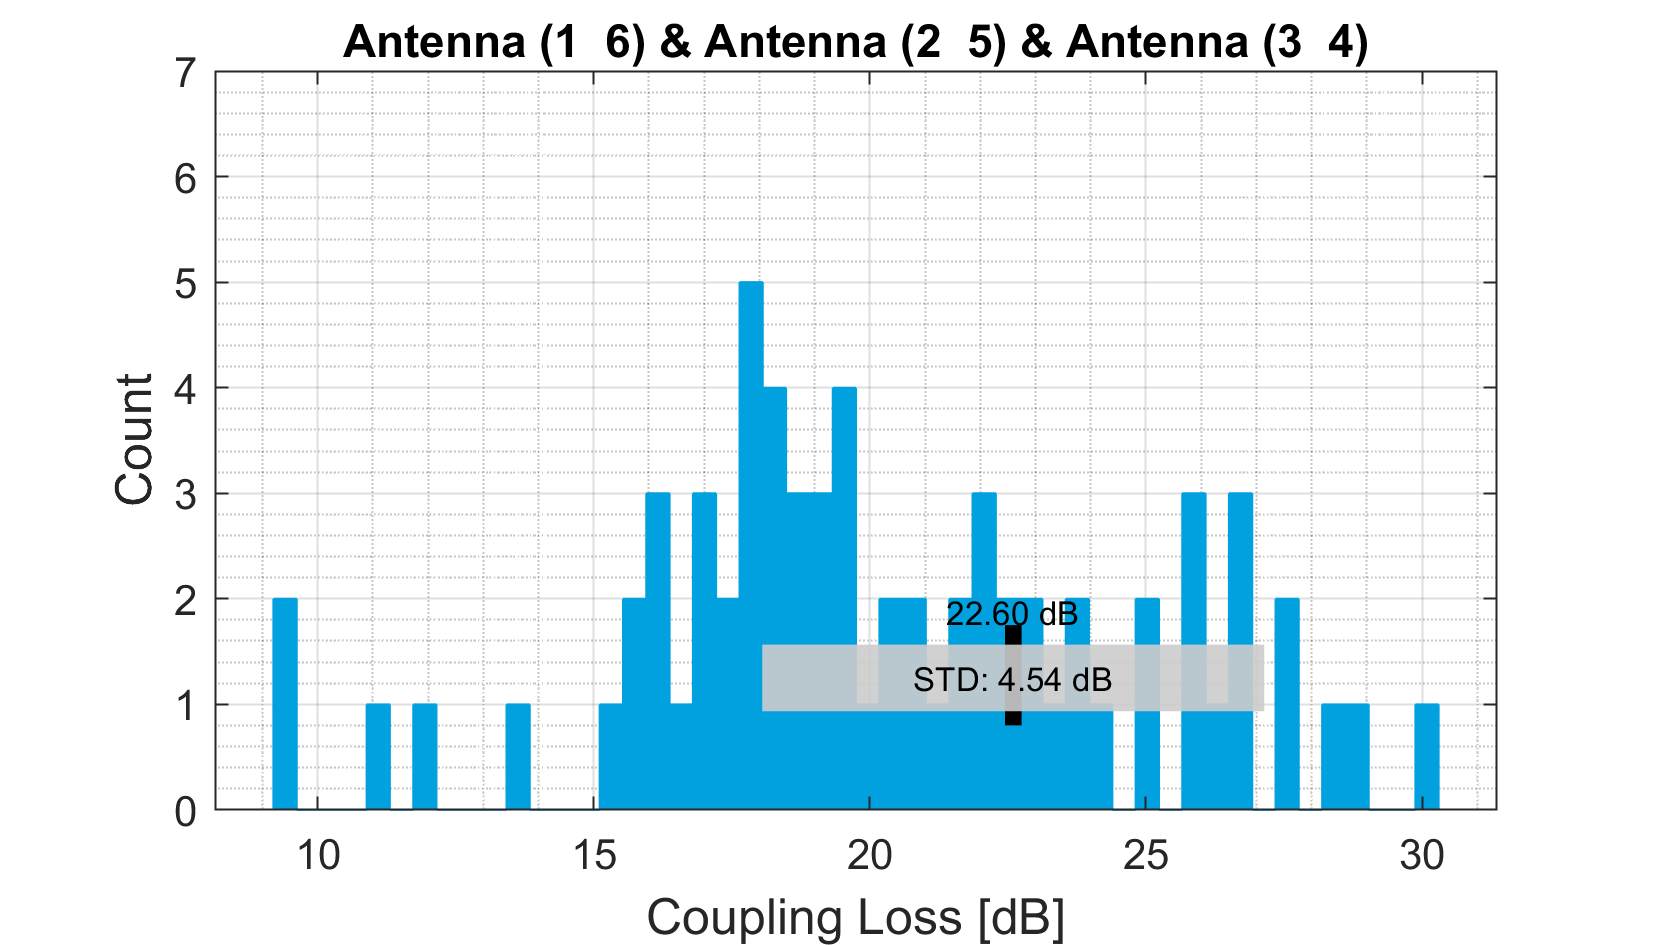
\includegraphics[scale = 0.37]{/Annex/Manual/plot15.png}}  
        \caption{Manual Measurements for optimization of antenna pair}
        \label{fig:three graphs}
\end{figure}




